\newpage
\section{ Árboles de Decisión y Bosques Aleatorios}
\noindent Sea un vector aleatorio $\textbf{x}$ con $p$ los datos de entrada, e $Y$ la variable respuesta. Supóngase también que se toman $n$ observaciones obteniéndose parejas $(\textbf{x}_i,y_i)$. De esta manera, tenemos que las $\textbf{x}_i\in \mathbb{R}^p$.

\noindent Los métodos de árbol son algoritmos divisivos, en los que se define una función de idoneidad, es decir, se establece un criterio con el cual una división es más idónea o no. Una vez conocida la división a realizar, se obtienen dos o más regiones (\emph{De ahora en adelante, serán separaciones binarias para la sencillez de los desarrollos.}). Este proceso de división se repite de manera iterativa sobre cada una de las regiones del espacio de observaciones en 

\noindent De esta manera, si se toma un método de árbol con separaciones o divisiones binarias, se obtiene un diagrama de árbol, en el que cada nodo es cada una de las regiones obtenidas en cada una de las separaciones, de esta manera, se obtiene una visión intuitiva del proceso del árbol y como ha ido avanzando.


\subsection*{Notación}
\begin{defi}
Se llama \emph{separación, partición o división} de índice $(j,s)$ \cite{Hastie 2001} a la separación que particiona el espacio inicial dado en las siguientes regiones $R_1,R_2$:
\begin{equation}
R_1=\lbrace \mathbf{x}_i \in \mathbb{R}^p/ x_{ij}>s\rbrace \quad R_2=\lbrace \mathbf{x}_i \in \mathbb{R}^p/ x_{ij}\leq s\rbrace
\end{equation}

\noindent Hay que tener en cuenta que esto sería el caso en el que la variable a separar $X_j$ sea continua, en caso, contrario, se puede definir la partición $(j,s)$ de la siguiente manera: 

\end{defi}

\begin{defi}
Se llama nodo de un árbol de decisión a cada una de las regiones resultantes tras aplicar una separación.
\end{defi}

\begin{defi}
Se llama nodo terminal de un árbol de decisión a las regiones finales en las que se ha particionado el espacio de observaciones. 
\end{defi}

\noindent En particular, los nodos terminales son las regiones en las que se ha particionado el espacio de observaciones. 










%Los métodos de árboles son un método divisivo, ya que tras aplicarlos, se obtiene una partición del espacio de observaciones $\mathbb{R}^p$ y luego en cada región del espacio se ajusta un modelo más simple, incluso una constante.\\


%La ventaja de este tipo de métodos es que son fácilmente interpretables, ya que pueden ser representados mediante un diagrama de tipo árbol. De esta manera, pueden ser utilizados según \textit{Brown et.al}.\cite{Brown 2004} tanto para análisis exploratorio, detectando características de grandes cantidades de datos, como para tareas de regresión y clasificación. \\ 
%Las  siguientes imágenes procedentes de \textit{Hastie et. al.}\cite{Hastie 2001} muestran el diagrama resultante tras dividir el espacio de observaciones mediante un árbol.
%
%\begin{figure}[h]
% \centering
%  \subfloat[División de $\mathbb{R}^p$]{
%   \label{f:división}
%    \includegraphics[width=0.4\textwidth]{Documentos Extra/Imagenes/Regiones árboles.png}}
%  \subfloat[Diagrama resultante]{
%   \label{f:diagrama arbol}
%    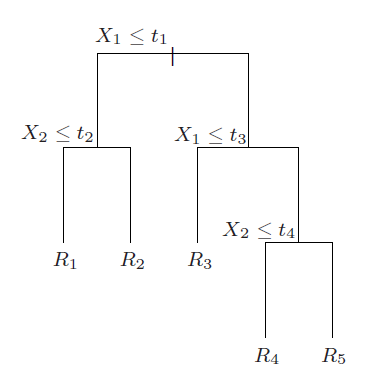
\includegraphics[width=0.4\textwidth]{Documentos Extra/Imagenes/Diagrama de arbol.png}}
% \caption{Representación de la división de $\mathbb{R}^p$ y el diagrama de árbol resultante}
% \label{f:MARC1}
%\end{figure}
%
%\noindent Otra ventaja de este tipo de métodos es que permite trabajar con conjuntos de datos en los que se estudian más variables en comparación de las observaciones, es decir, $p > n$. Por ejemplo, el ejemplo que desarrollan \textit{Díaz-Uriarte y De Andrés} \cite{Diaz 2006}, en el que trabajan con un microarray genético. 
%
%\noindent Otro de los problemas que surgen del propio planteamiento del modelo en sí es que el algoritmo para obtener las divisiones están diseñados para sobreajustarse a los datos por tanto, surgen métodos como la ``poda''. Se desarrollará más adelante, pero el idea es poder modelizar toda la variación del conjunto de entrenamiento. 

\newpage
\subsection{Árboles de Regresión}
\noindent Sea un vector aleatorio $\textbf{x}$ de variables predictoras como antes y una variable $Y$ de respuesta. 
Supóngase que queremos dividir el espacio de observaciones en $M$ regiones, $R_1,\ldots R_M$, se puede modelar en cada una de las regiones como la constante $c_m$. Por tanto teniendo en cuenta, la siguiente definición. 
\begin{equation}
\mathbf{1}_m(\textbf{x})=
\begin{cases}
0\quad& \text{si } x\notin R_m\\
1\quad& \text{si } x\in R_m\\
\end{cases}
\end{equation}
Es decir, la función $\mathbf{1}(\textbf{x})$ es la función característica de la región $R_m$, por tanto puede construirse el siguiente predictor:
\begin{equation}
f(\textbf{x})=\sum_{m=1}^M c_m \mathbf{1}_m(\textbf{x})
\end{equation}

\noindent Un problema que surge es que en principio cualquier tipo de región sería aceptable. Esta libertad llevaría a tener que explorar cualquier región posible, lo cual no es viable computacionalmente hablando. Es por ello, que se toma un tipo de división en particular, las divisiones binarias en semihiperplanos. De esta manera, se generan regiones que son rectángulos de altas dimensiones. 


\noindent Si se toma como criterio de ajuste los mínimos cuadrados obtendremos que $\hat{c}_m=ave(y_i|x_i\in R_m)$, ya que es la media condicional de la y sabiendo el valor de x. 

\noindent Para obtener las regiones se toma una variable $X_j$ y un valor de separación $s$, es decir, cada separación se puede identificar con una pareja $(j,s)$. 
Por ejemplo, supóngase una separación $(j,s)$ entonces se generan dos regiones del espacio de las observaciones $R_1, R_2$. 
\begin{equation}
R_1=\lbrace\textbf{x}|X_j\leq s\rbrace\quad R_2=\lbrace\textbf{x}|X_j > s\rbrace 
\end{equation}

\noindent Hay que establecer un criterio para elegir que separaciones se deben hacer en particular, para ello se utilizan los mínimos cuadrados:
\begin{equation}
\min_{j,s}\left[\min_{c_1}\sum_{x_i\in R_1}(y_i-c_1)^2+\min_{c_2}\sum_{x_i\in R_2}(y_i-c_2)^2\right]
\end{equation}

\noindent Es decir, teniendo en cuenta que se va a predecir el valor de la variable respuesta $y_i$ como una constante, la función anterior es la función $RSS$ 

\noindent Las mejores estimaciones de las constantes según el criterio de los mínimos cuadrados sería la media de las respuestas dentro de las regiones, es decir: 
\begin{equation}
\hat{c}_m=\dfrac{1}{n_m}\sum_{\textbf{x}_i\in R_m} y_i
\end{equation}

\noindent De esta manera, con estas estimaciones de las constantes de cada región, es posible encontrar la mejor división del espacio de observaciones. 

\noindent Se puede conseguir la mejor pareja $(j,s)$ fijando la $j$-ésima variable, encontrar el mejor valor $s$ para cada variable, de manera sencilla.

\begin{defi}
Diremos que un algoritmo es \textit{voraz} o \textit{greedy} si en cada paso local busca la solución óptima. 
\end{defi}

\noindent En cada paso, el árbol busca en cada paso la división que mayor disminución produce en el $RSS$, por tanto, se utiliza un algoritmo voraz. 

\noindent El siguiente problema es controlar la complejidad del modelo, en particular, cuanto debe crecer el árbol, ya que un árbol demasiado grande  puede pecar de problemas de sobre ajuste. 

\noindent La estrategia más común es tener un criterio de parada, en particular hacer crecer un árbol grande $T_0$ y ``podarlo''   cuando en los nodos terminales tenga menos de $5$ individuos según \textit{Díaz-Uriarte y De Andrés} \cite{Diaz 2006}, además este es el valor por defecto que otorga la librería de  \texttt{R, randomForest}. Si se hace más grande esto provoca que los árboles sean más pequeños.


\begin{defi}
Llamaremos tamaño de un árbol $T$ y se denota por $|T|$ al número de nodos terminales, es decir, al número de regiones en las que se particiona el espacio de observaciones.
\end{defi}

\noindent Se puede entonces definir el error cuadrático medio de un nodo de un árbol de la siguiente manera:
\begin{equation}
Q_m(T)= \dfrac{1}{n_m}\sum_{\textbf{x}_i\in R_m}(y_i- \hat{c}_m)^2
\end{equation}

\noindent Con la anterior función y el concepto del tamaño del árbol, el cual está directamente relacionado con la complejidad del modelo, se puede establecer un criterio para un árbol que penalice la complejidad:
\begin{equation} \label{Eq Cost-Complexity}
C_{\alpha}(T)=\sum_{m=1}^{|T|}n_m Q_m(T) + \alpha|T|
\end{equation}

\noindent El valor de $\alpha$ es un parámetro que es elegido y su valor hace que se penalice más o menos la complejidad del modelo. A valores más altos, tendremos un modelo menos complejo y con $\alpha = 0$ es el modelo obtenido por mínimos cuadrados.

\noindent El objetivo es encontrar el árbol de menor tamaño para cada $\alpha$ que minimice la función \eqref{Eq Cost-Complexity}. Para ello se empieza con el árbol completo o con un árbol inicial $T_0$ y se van juntando regiones de tal manera que el aumento provoquen sobre la función $\sum_{m=1}^{|T|}n_m Q_m(T)$, sea el menor posible, resultando en una secuencia de árboles entre los cuales se encuentra el que minimiza la función $C_{\alpha}(T)$ para un $\alpha $ determinado. 

\noindent Para llevar a cabo el proceso completo, se deben aplicar procesos de validación cruzada, por ejemplo  en \textit{Divakaran S.}\cite{Divakaran 2022} o en \textit{James G. et.al.} \cite{James 2013} se detalla el algoritmo de Breiman. En este algoritmo se  usa la validación cruzada de K-folds, \textit{(Para más detalles sobre dicho proceso, léase la sección 7.10 de Hastie et.al \cite{Hastie 2001} o la sección 5.1.3 James et.al. \cite{James 2013})} para poder elegir el $\alpha$ que minimice el error.


\subsection{Árboles de Clasificación}
\noindent Gran parte de lo anterior se puede detallar de manera análoga a los árboles de regresión. En esencia, un árbol de clasificación es un conjunto de funciones discriminantes utilizadas de manera recurrente obteniéndose en el caso óptimo una partición del espacio de observaciones en el que cada región contiene observaciones que pertenecen únicamente a una categoría.



\noindent A partir de este punto, la variable respuesta será una variable categórica con valores posibles $1,\ldots, K$.

\noindent Sea un nodo $m$ que representa una de las regiones $R_m$ en las que se han particionado el espacio con $n_m$ observaciones en ella. Entonces, la proporción de observaciones que son de la clase $k$-ésima en el nodo $m$ es:
\begin{equation}
\hat{p}_{mk}=\dfrac{1}{n_m}\sum_{\textbf{x}_i \in R_m}\mathbf{1}(y_i=k)
\end{equation}

\noindent En cada región $R_m$ se tomará como predicción la respuesta cuya $\hat{p}_{mk}$ sea máxima. 

\noindent Una vez definido esto se ha de definir el concepto de pureza de un nodo
\begin{defi}
Diremos que un nodo es \textit{puro u homogéneo} si todas las observaciones que pertenecen a la región establecida por dicho nodo pertenecen a la misma clase. En caso contrario se dice que el nodo es \textit{impuro}
\end{defi}

\noindent Es este concepto de la impureza lo que  permite establecer un criterio para realizar las divisiones del espacio. Es decir, en cada paso se elegirá la división $(j,s)$ que produzca los nodos más puros. 

\noindent Teniendo en cuenta la definición que dimos de $\hat{p}_{mk}$ se pueden dar distintas medidas de la impureza de un nodo. Como detallan tanto \textit{Hastie et.al}\cite{Hastie 2001} como \textit{Brown et.al.}\cite{Brown 2004}

\begin{defi}
\noindent Sea un nodo y su región correspondiente, $R_m$, sea además $k$ el valor para el cual $\hat{p}_{mk}$ es mayor que el resto, se define el \textit{Error de Clasificación errónea} como:
\begin{equation}
\dfrac{1}{n_m}\sum_{\textbf{x}_i\in R_m}\mathbf{1}(y_i\neq k)=1-\hat{p}_{mk}
\end{equation}
\end{defi}
\noindent Es la proporción de observaciones en el nodo que no tienen la misma categoría que el más frecuente.
Esta medida no es la más usada debido a que no es derivable y no es muy sensible a los cambios.  

\noindent Por otro lado, el \textit{índice Gini} no solo tiene en cuenta la proporción máxima o la categoría máxima sino que da una medida de la varianza total entre las $K$ categorías posibles. Lo cual arroja una mejor visión de la pureza de cada nodo. 
\begin{defi}
Se llama \textit{índice Gini} a la siguiente medida:
\begin{equation}
G=\sum_{k=1}^K \hat{p}_{mk}(1-\hat{p}_{mk})
\end{equation}
\end{defi}

\noindent Otra medida alternativa sería la 
\textit{entropía} del nodo que se define 
\begin{defi}
Se llama \textit{entropía} de un nodo $m$ o de una región $R_m$ a:
\begin{equation}
D= - \sum_{k=1}^K \hat{p}_{mk} log(\hat{p}_{mk})
\end{equation}
\end{defi}
\noindent Ambas medidas son bastante similares. 

\noindent El algoritmo para construirlos es análogo al de los árboles de regresión. Tomando la medida de impureza o pureza que se desee se puede construir un árbol de clasificación teniendo en cuenta que el error de clasificación produce de manera general según \textit{James et.al.} \cite{James 2013} árboles con una precisión mayor. 

\noindent Aunque en la mayoría de casos según \textit{Brown et.al}\cite{Brown 2004} lo que ocurre al utilizar distintas medidas es que los modelos no obtienen errores de predicción muy alejados, sin embargo, pueden provocar que los modelos tengan complejidades muy diferentes. 


\subsection{Bosques Aleatorios}

\noindent Los bosques aleatorios y otros métodos de juntar árboles de decisión son maneras de solventar ciertos problemas que tienen los árboles de decisión individuales como puede ser la precisión o la dependencia del conjunto de datos, ya que una pequeña variación en estos puede provocar grandes cambios. 


\noindent Durante esta sección no se detallarán los métodos de construcción de cada árbol individual ya que se han descrito anteriormente y se hará referencia a ellos como árboles simplemente. 

\noindent Estos métodos se basan en el  Bagging y el Bootstrap, ambos métodos se pueden utilizar cuando la cantidad de datos es pequeña o cuando el modelo sufre de \textit{sobreajuste}. 

\noindent El proceso de Bagging tiene como base el hecho de que si se tienen $n$ observaciones independientes de una población con varianza $\sigma^2$ entonces la media de dichas observaciones tendrá varianza $\frac{\sigma^2}{n}$, es decir, tomar la media de distintas observaciones provoca una disminución en la varianza. 


\noindent De esta manera, partiendo de un conjunto inicial de datos, se toman muestras aleatorias de los mismos y se entrenan distintos modelos para luego hacer la media entre todos los modelos. Es decir, se hace un muestreo aleatorio entre las $n$ observaciones obteniendo $B$ conjuntos de entrenamiento distintos y se estiman los predictores $\hat{f}_1(\textbf{x}),\ldots, \hat{f}_B(\textbf{x})$ y el modelo final es:
\begin{equation}
\hat{f}_{bag}(\textbf{x})=\dfrac{1}{B}\sum_{b=1}^B \hat{f}_b(\textbf{x})
\end{equation}

\noindent Esto se puede aplicar perfectamente al caso de la modelización mediante árboles de decisión aunque esta técnica puede ser útil para cualquier tipo de modelos. 

\noindent En este caso, estamos utilizando en cada división de los árboles todos los predictores, sin embargo, cuando una variable tiene demasiada importancia a la hora de predecir la variable de respuesta, la mayoría de divisiones en casi todos los árboles van a utilizar ese predictor, ya que va a provocar mejoras sustanciales en el $RSS$ o en el \textit{índice Gini} dependiendo del tipo de árbol. 

\noindent Para evitar dicho problema, en el algoritmo del bosque aleatorio se toma en cada división no el total de predictores, si no una muestra aleatoria de tamaño $m$ que habitualmente es $m=\sqrt{p}$ de esta manera, se puede tener modelos con mayor variedad. 

\noindent En \textit{Biau G. y Scornet E.}\cite{Biau 2016} se detalla el algoritmo para la creación de un bosque aleatorio. 
En este algoritmo se deben definir los siguientes parámetros:
\begin{itemize}
\item $\mathcal{M}$: Número de árboles que se incluirán en el bosque aleatorio. 
\item $\mathtt{m}_{\mathtt{try}}$, es el número de predictores que entre los cuales se pueden usar en cada división del espacio. 
\item $a_n$: Número de observaciones del conjunto de entrenamiento que se utilizarán para entrenar cada árbol. 
\end{itemize}

\noindent El algoritmo en sí es el siguiente: 
\hrule
\textbf{for } $j=1\ldots \mathcal{M} $ \textbf{do:}
\begin{itemize}
\item Se extrae de manera uniforme un subconjunto de tamaño $a_n$ del conjunto de observaciones de entrenamiento. 
\item Se extrae aleatoriamente un conjunto de predictores posibles $\mathcal{M}_{try}$ de tamaño $\mathtt{m}_{\mathtt{try}}$ y se construye el árbol, utilizando como posibles  predictores únicamente los que están en el conjunto $\mathcal{M}_{try}$
\end{itemize}
\hrule

\noindent Para hacer la predicción para una nueva observación $\textbf{x}_0$, hay que calcular la predicción para cada uno de los $\mathcal{M}$ árboles. Una vez calculadas en el caso de que la variable respuesta sea numérica se hace la media de todas las predicciones. Si por el contrario, $Y$ es una variable categórica, se toma como predicción aquella que haya salido con mayor frecuencia, lo que se llama predicción por \textit{voto de mayoría}.

\noindent En el artículo de \textit{Biau, G y Scornet, E.} \cite{Biau 2016} se detallan más en profudidad las distintas características de estos modelos. En particular, se detalla la necesidad de utilizar modelos simplificados para poder analizar las características de los bosques aleatorios. Estos pueden ser los bosques puramente aleatorios que hace particiones totalmente aleatorias sin tener un criterio de acuerdo a los datos y otras modificaciones.

\noindent En particular, \textit{Breiman L.} \cite{Breiman 2004}, utiliza los siguientes resultados empíricos para poder analizar la consistencia y el ratio de convergencia de los bosques aleatorios utilizando un modelo más simplificado de los mismos. 
\begin{itemize}
\item El muestreo aleatorio que se hace del conjunto de entrenamiento no tiene efecto en el ratio de error.
\item Si para conseguir una partición en la que únicamente en cada nodo haya una sola observación se utiliza la mediana de las variables aleatorias esto no tiene efecto en el ratio de error. 
\item Hacer divisiones sin tener en cuenta las clases que conocemos, sí aumenta el error.
\end{itemize}

\noindent De esta manera, establece un modelo simplificado en el las variables predictoras se pueden dividir en dos grupos, las variables fuertes $\mathcal{S}$ y las variables débiles $\mathcal{W}$. Las variables fuertes son las que tienen una influencia directa sobre las predicciones y las débiles se pueden interpretar como ruido.

\noindent Teniendo en cuenta lo anterior, las variables aleatorias fuertes se dividen en la mediana, mientras que si es débil se toma un valor aleatorio para la división.  

\noindent Como resultado de dichas modificaciones \textit{Breiman, L.} \cite{Breiman 2004} concluye que el ratio de convergencia es $\mathcal{O}\left(n^{\left(\frac{-0.75}{|\mathcal{S}|log 2+0.75}\right)}\right)$.\\
Por tanto, el ratio de error depende del número de variables fuertes. 

 